\documentclass[12pt, a4paper, oneside]{article}
\usepackage{amsmath, amsthm, amssymb, graphicx}
\usepackage{geometry}
\usepackage[bookmarks=true, colorlinks, citecolor=blue, linkcolor=black]{hyperref}
\usepackage{ctex}
\usepackage{tikz}
\usetikzlibrary{patterns}

\geometry{
    a4paper, % 页面尺寸
    left=3cm, % 左边距
    right=3cm, % 右边距
    top=3cm, % 上边距
    bottom=3cm, % 下边距
}

\title{Computer Vision}
\author{Lingjie Zhang}
\date{2024 SS}

\renewcommand{\contentsname}{Contents}

% 修改图片标签名称为 "img"
\renewcommand{\figurename}{Figure}

% 修改表格标签名称为 "table"
\renewcommand{\tablename}{Table}

% 在每个章节重置图片计数器
\counterwithin{figure}{section}

\begin{document}
\maketitle

\centering
\textbf{This course is based on the lecture EI70110 of Technical University of Munich}

\raggedright

\tableofcontents
\pagenumbering{roman}
\newpage
\pagenumbering{arabic}


\section{Wissenswertes über Bilder}

\subsection{Darstellung von Bildern}
\subsubsection*{Von Farbbild zum Intensitätsbild}
\begin{itemize}
    \item Farbbilder bestehen aus mehreren Kanälen
    \item In diesem Kurs ausschließlich Graustufenbilder
\end{itemize}

\begin{figure}[htbp]
    \centering
    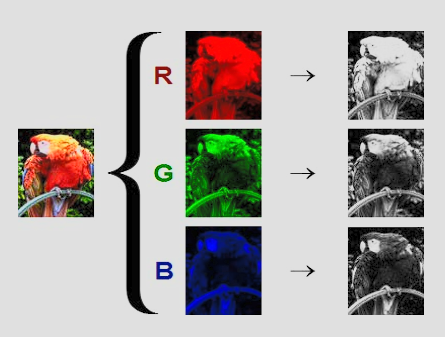
\includegraphics[scale=0.8]{../img/1-1.png}
    \caption{RBG image}
    \label{img/1-1}
\end{figure}

\subsubsection*{Kontinuierliche und diskrete Darstellung}
\begin{itemize}
    \item \textbf{Kontinuierliche} Darstellung als Funktion zweier Veränderlicher (zum Herleiten von Algorithmen) 
    $I: \mathbb{R}^2\supset\Omega\to\mathbb{R}, (x,y)\mapsto I(x,y)$
    \item Häufige Annahmen:
    \begin{itemize}
        \item $I$ differenzierbar
        \item $\Omega$ einfach zusammenhängend und beschränkt
    \end{itemize}
    \item Diskrete Darstellung als Matrix $I\in \mathbb R^{m\times n}$
    
    Eintrag $I_{k,l}$ entspricht dem Intensitätswert
    \item Skalierung typischerweise zwischen [0, 255] oder [0, 1]
\end{itemize}

\begin{table}[h]
\centering
\begin{tabular}{|c|}
\hline
VGA: 480$\times$ 640  Pixel (ca. 0.3 Megapixel) \\
\hline
HD: 720$\times$ 1280  Pixel (ca. 1.0 Megapixel) \\
\hline
FHD:  1080$\times$ 1920  Pixel (ca. 2.1 Megapixel) \\
\hline
\end{tabular}
\label{tab:table_label}
\end{table}

\begin{figure}[htbp]
    \centering
    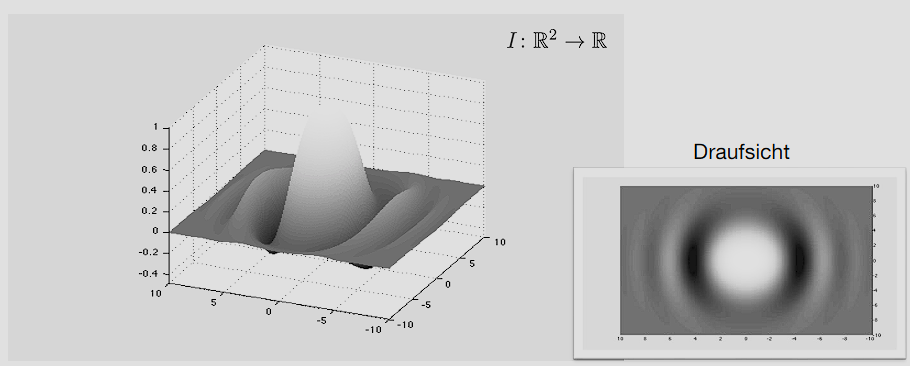
\includegraphics[scale=0.7]{../img/1-2.png}
    \caption{Graph einer Funktion}
    \label{img/1-2}
\end{figure}

\begin{figure}[htbp]
    \centering
    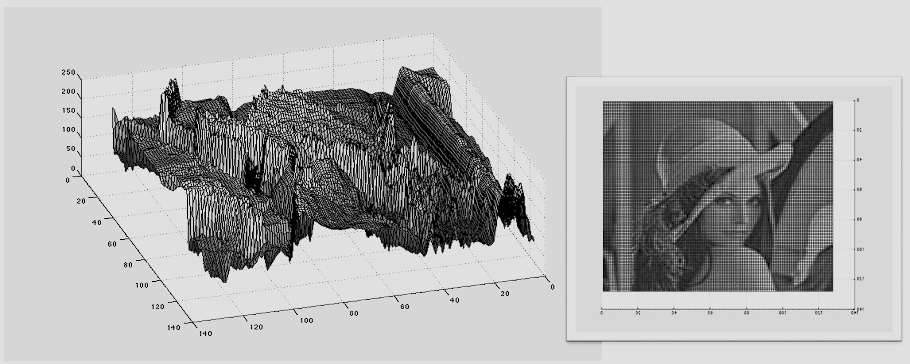
\includegraphics[scale=0.7]{../img/1-3.png}
    \caption{Graph eines Fotos}
    \label{img/1-3}
\end{figure}

\subsubsection*{Diskretes Abtasten}
\begin{itemize}
    \item Abtasten eines eindimensionalen Signals
    $$S\{f(x)\}=(...,f(x-1),f(x),f(x+1),...)$$
    \item Abtasten eines Bildes \\
    $$
    S\{I(x,y)\}=
    \begin{bmatrix}
    \ddots & \vdots & \vdots & \vdots & \\\
    \cdots & I(x-1,y-1) & I(x-1,y) & I(x-1,y+1) & \cdots\\
    \cdots & I(x,y-1) & I(x,y) & I(x,y+1) & \cdots\\
    \cdots & I(x+1,y-1) & I(x+1,y) & I(x+1,y+1) & \cdots\\
    & \vdots & \vdots & \vdots & \ddots
    \end{bmatrix}
    $$
\end{itemize}

\subsubsection*{Diskrete Darstellung/Matrixdarstellung}
\begin{itemize}
    \item Annahme: Ursprung links oben
    \item Matrixeintrag ist $I_{k,l}=S\{I(0,0)\}_{kl}$
\end{itemize}
\begin{figure}[htbp]
    \centering
    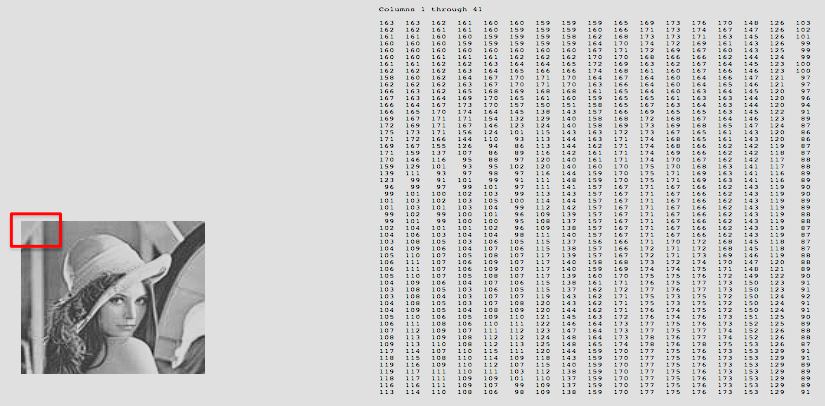
\includegraphics{../img/1-4.png}
    \caption{Diskrete Darstellung/Matrixdarstellung}
    \label{img/1-4}
\end{figure}

\subsubsection*{Zusammenfassung}
\begin{itemize}
    \item Bilder in Grautönen
    \item Bilder als Matrizen
    \item Bilder als glatte Funktionen
\end{itemize}

\newpage

\subsection{Bildgradient}
\subsubsection{Der Gradient eines Bildes}
\begin{figure}[htbp]
    \centering
    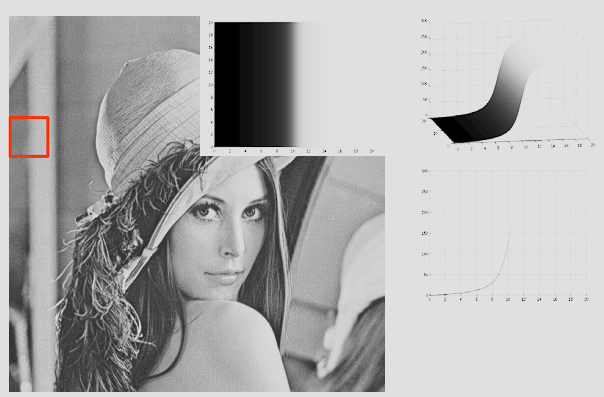
\includegraphics{../img/1-5.png}
    \caption{Der Gradient eines Bildes}
    \label{img/1-5}
\end{figure}
Kanten sind starke lokale Änderungen der Intensität. Lokale Änderungen werden durch den Gradienten beschrieben.
$$
    \nabla I(x,y)=\begin{bmatrix}
    \frac{\partial}{\partial x}I(x,y) \\
    \frac{\partial}{\partial y}I(x,y)
    \end{bmatrix}
$$

\paragraph{Wie schätzt man den Gradienten?}
Gegeben ist das Bild in diskreter Form $I\in \mathbb R^{m\times n}$.
$$
    \frac{\partial}{\partial x} I(x,y)\approx I(x+1,y)-I(x,y)
$$
$$
    \frac{\partial}{\partial y}I(x,y)\approx I(x,y+1)-I(x,y)
$$

\subsubsection{Diskretes und kontinuierliches Signal}
\paragraph*{Interpolation}
Vom diskreten Signal $f[x]=S\{f(x)\}$ zum kontinuierlichen Signal $f(x)$. Interpoliertes Signal ist Faltung der Abtastwerte mit dem Interpolationsfilter.
$$
    f(x)\approx \sum_{k=-\infty}^{\infty}f[k]h(x-k)=:f[x]*h(x)
$$

\paragraph*{Interpolationsfilter}
Diskretes Signal: $f[x]=S\{f(x)\}$. Kontinuierliches Signal: $f(x)\approx f[x]*h(x)$.
\begin{itemize}
    \item Gaußfilter: $h(x)=g(x)$
    \item Ideales Interpolationsfilter: $h(x)=\operatorname{sinc}(x)$
    \item Damit gilt: $f[x]*h(x)=f(x)$
\end{itemize}

\begin{figure}[htbp]
    \centering
    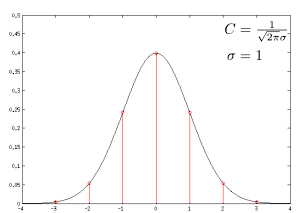
\includegraphics[scale=1]{../img/1-6.png}
    \caption{$g(x)=Ce^{\frac{-x^2}{2\sigma^2}}$}
    \label{img/1-6}
\end{figure}
\begin{figure}[htbp]
    \centering
    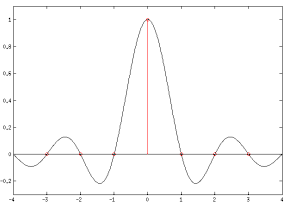
\includegraphics[scale=1]{../img/1-7.png}
    \caption{$sinc(x)=\frac{sin(\pi x)}{\pi x}, sinc(0):=1$}
    \label{img/1-7}
\end{figure}

\subsubsection{Die diskrete Ableitung}
\paragraph*{Mit Hilfe des rekonstruierten Signals}
\begin{itemize}
    \item Algorithmisch
    \begin{enumerate}
        \item Rekonstruktion des kontinuierlichen Signals
        \item Ableitung des kontinuierlichen Signals
        \item Abtastung der Ableitung
    \end{enumerate}
    \item Herleitung
    \begin{itemize}
        \item $f'(x)\approx \frac{d}{dx}(f[x]*h(x))$\\$f[x]*h'(x)$
        \item $f'[x]=f[x]*h'[x]$\\$=\sum\limits _{k=-\infty}^{\infty}f[x-k]h'[k]$
    \end{itemize}
\end{itemize}

\begin{figure}[htbp]
    \centering
    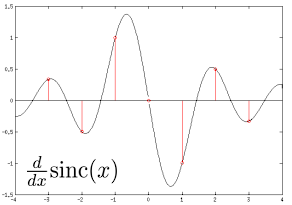
\includegraphics[scale=1]{../img/1-8.png}
    \caption{Sinc-Funktion(Langsames Abklingen)}
    \label{img/1-8}
\end{figure}
\begin{figure}[htbp]
    \centering
    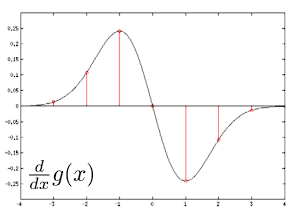
\includegraphics[scale=1]{../img/1-9.png}
    \caption{Gaußfilter(Schnelles Abklingen)}
    \label{img/1-9}
\end{figure}

\subsubsection{Zweidimensionale Rekonstruktion}
\paragraph*{Separables 2D-Gaußfilter}
2D-Rekonstruktion: $I(x,y)\approx I[x,y]*h(x,y)=\sum\limits _{k=-\infty}^{\infty}\sum\limits_{l=-\infty}^{\infty}I[k,l]g(x-k)g(y-l)$
\begin{figure}[htbp]
    \centering
    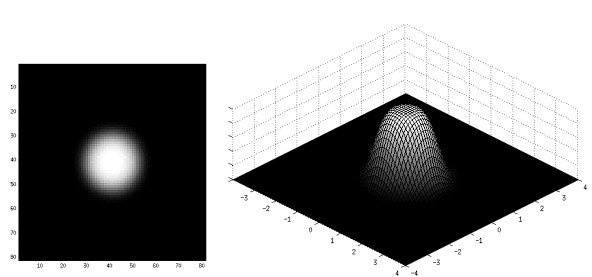
\includegraphics[scale=1]{../img/1-10.png}
    \caption{$h(x,y):=g(x)g(y)$}
    \label{img/1-10}
\end{figure}

\subsubsection{Zweidimensionale Ableitung}
\paragraph*{Ausnutzen der Separabilität}
Ableitung in x-Richtung
\begin{align*}
    \frac{d}{dx}I(x,y) & \approx I[x,y]*(\frac{d}{dx}h(x,y)) \\
    & = \sum\limits_{k=-\infty}^{\infty} \sum\limits_{l=-\infty}^{\infty}I[k,l]g'[x-k]g(y-l)
\end{align*}
\begin{align*}
    S\{\frac{d}{dx}I(x,y)\} & = I[x,y]*g'[x]*g[y] \\
    & = \sum\limits_{k=-\infty}^{\infty} \sum\limits_{l=-\infty}^{\infty}I[x-k,y-l]g'[k]g[l]
\end{align*}

\subsubsection{Endliche Approximation des Gaußfilters}
\paragraph*{Normierung des endlichen Filters}
\begin{itemize}
    \item In der Praxis wird die unendliche Summe durch wenige Summanden approximiert
    \item Wie wählt man eine geeignete Gewichtung $C$ des Gaußfilters $g(x)=Ce^{\frac{-x^2}{2\sigma^2}}$?
    \item Interpoliertes Signal: $f(x)\approx \sum\limits_{k=-\infty}^{\infty}f[k]g(x-k)$
    \item Abgetastetes interpoliertes Signal: $f[x]\approx \sum\limits_{k=-\infty}^{\infty}f[x-k]g[k]$
    \item Approximation durch endliche Summe: $f[x]\approx \sum\limits_{k=-n}^{n}f[x-k]g[k]$
    \item Die endliche Approximation von $f[x]$ ist eine gewichtete Summe der Werte $f[x-n],...,f[x+n]$ mit den Gewichten $g[n],...,g[-n]$
    \item Normierungskonstante $C$ so gewählt, dass sich alle Gewichte zu 1 addieren
    \item Wähle $C=\frac{1}{\sum\limits_{-n\le k\le n}e^{\frac{-k^2}{2\sigma^2}}}$
\end{itemize}

\subsubsection{Sobel-Filter}
\paragraph*{Herleitung}
\begin{itemize}
    \item Approximation von $S\{\frac{d}{dx}I(x,y)\}=I[x,y]*g'[x]*g[y]=\sum\limits_{k=-\infty}^{\infty}\sum\limits_{l=-\infty}^{\infty}I[x-k,y-l]g'[k]g[l]$ durch endliche Summe $\sum\limits_{k=-1,0,1}^{}\sum\limits_{l=-1,0,1}^{}I[x-k,y-l]g'[k]g[l]$
    \item Daraus folgt der Normierungsfaktor $C=\frac{1}{1+2e^{-\frac{1}{2\sigma^2}}}$
    \item Für die Wahl $\sigma = \sqrt[]{\frac{1}{2\log 2}}$ ergeben sich somit die Werte
    \begin{align*}
        & g[-1]=\frac{1}{4}; g[0]=\frac{1}{2}; g[1]=\frac{1}{4} \\
        & g'[-1]=\frac{1}{2}\log 2; g'[0]=0; g'[1]=-\frac{1}{2}\log 2\;\;\;\;(\frac{1}{2}\log 2\approx 0.35)
    \end{align*}
    \item Aus praktischen Gründen sind ganzzahlige Filterkoeffizienten erwünscht
    \item Für das Detektieren von Intensitätsunterschieden ist ein Vielfaches des Gradienten ausreichend
\end{itemize}

\begin{figure}[htbp]
    \centering
    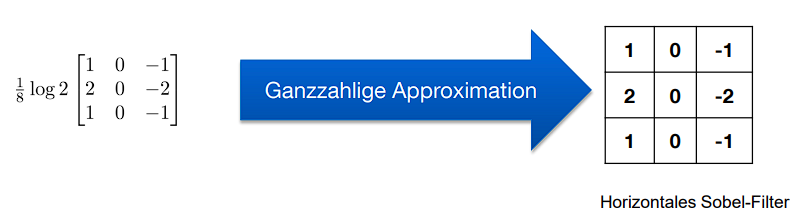
\includegraphics[scale=1]{../img/1-11.png}
    \label{img/1-11}
\end{figure}

\paragraph*{Beispiel}
\begin{figure}[htbp]
    \centering
    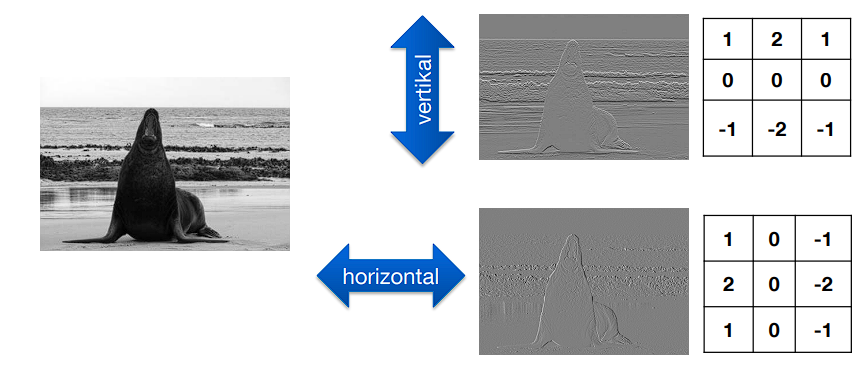
\includegraphics[scale=0.6]{../img/1-12.png}
    \caption{Sobel-Filterung}
    \label{img/1-12}
\end{figure}

\subsubsection{Zusammenfassung}
\begin{itemize}
    \item Der Bildgradient ist ein wichtiges Werkzeug für die Bestimmung von lokalen Intensitätsänderungen
    \item Diskrete Ableitung wird durch Differenzieren des interpolierten Signals berechnet
    \item Sobel-Filter sind ganzzahlige Approximation eines Vielfachen des Gradienten 
\end{itemize}

\subsection{Merkmalspunkte-Ecken und Kanten}
\subsubsection{Ecken und Kanten}
\paragraph*{...liefern markante Bildmerkmale}
\begin{itemize}
    \item Bestimmung von Konturen
    \item Berechnungen von Bewegungen in Bildsequenzen
    \item Schätzen von Kamerabewegung
    \item Registrierung von Bildern
    \item 3D-Rekonstruktion
\end{itemize}

\subsubsection{Harris Ecken- und Kantendetektor}
\paragraph*{Änderung des Bildsegments in Abhängigkeit der Verschiebung}
\begin{figure}[htbp]
    \centering
    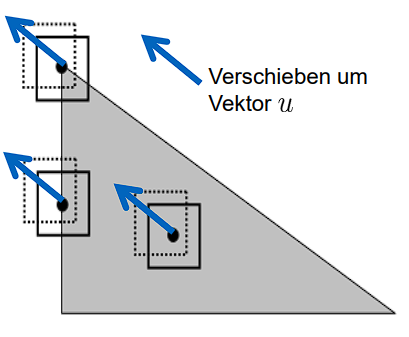
\includegraphics[scale=1]{../img/1-13.png}
    \label{img/1-13}
\end{figure}
\begin{itemize}
    \item Ecke: Verschiebung in jede Richtung bewirkt Änderung
    \item Kante: Verschiebung in jede bis auf genau eine Richtung bewirkt Änderung
    \item Homogene Fläche: Keine Änderung, egal in welche Richtung
\end{itemize}
\paragraph*{Formelle Beschreibung der Änderung}
\begin{itemize}
    \item Position im Bild: 
    $x=\begin{bmatrix}
        x_1 \\
        x_2
    \end{bmatrix},\;\;\;\;
    I(x)=I(x_1,x_2)$
    \item Verschiebungsrichtung: $u=\begin{bmatrix}
        u_1 \\
        u_2
    \end{bmatrix}$
    \item Änderung des Bildsegments:
    $$
    S(u)=\int_W (I(x+u)-I(x))^2dx
    $$
    \item Differenzierbarkeit von $I$:
    $$
    \lim_{u\to 0}\frac{I(x+u)-I(x)-\nabla I(x)^\top u}{||u||}=0
    $$
\end{itemize}
\paragraph*{Approximation der Änderung}
\begin{itemize}
    \item Folgerung aus Differenzierbarkeit: $I(x+u)-I(x)=\nabla I(x)^\top u + o(||u||)$
    \item Restterm $o(||u||)$ mit der Eigenschaft $\lim_{u\to 0}o(||u||)/||u||=0$
    \item Approximation für kleine Verschiebungen: $I(x+u)-I(x)\approx \nabla I(x)^\top u$
    \item Approximation der Änderung im Bildsegment:
    $$
    S(u)=\int_W(I(x+u)-I(x))^2dx\approx\int_W(\nabla I(x)^\top u)^2dx
    $$
\end{itemize}
\paragraph*{Die Harris-Matrix}
\begin{itemize}
    \item Ausmultiplizieren des Integrals:
    $$
    S(u)=\int_W(\nabla I(x)^\top u)^2dx=u^\top (\int_W \nabla I(x)\nabla I(x)^\top dx)u
    $$
    \item Harris-Matrix: $G(x)=\int_W \nabla I(x)\nabla I(x)^\top ds$
    $$\nabla I(x)\nabla I(x)^\top =\begin{bmatrix}
        (\frac{\partial}{\partial x_1}I(x))^2 & \frac{\partial}{\partial x_1}I(x)\frac{\partial}{\partial x_2}I(x) \\
        \frac{\partial}{\partial x_2}I(x)\frac{\partial}{\partial x_1}I(x) & (\frac{\partial}{\partial x_2}I(x))^2
    \end{bmatrix}
    $$
    \item Approximative Änderung des Bildsegments:
    $$
    S(u)\approx u^\top G(x)u
    $$
\end{itemize}

\paragraph*{Eigenwertzerlegung}
\begin{itemize}
    \item Eigenwertzerlegung der Harris-Matrix:
    $$
    G(x)=\int_W\nabla I(x)\nabla I(x)^\top dx=V \begin{bmatrix}
        \lambda_1 & \\
         & \lambda_2
    \end{bmatrix}
    V^\top
    $$
    mit $VV^\top =I_2$ und den Eigenwerten $\lambda_1\le \lambda_2\le 0$
    \item Änderung in Abhängigkeit der Eigenvektoren: $V=[v_1,v_2]$
    $$
    S(u)\approx u^\top G(x)u=\lambda_1(u^\top v_1)^2+\lambda_2(u^\top v_2)^2
    $$
\end{itemize}

\paragraph*{Art des Merkmals in Abhängigkeit der Eigenwerte}
\begin{itemize}
    \item Beide Eigenwerte positive
    \begin{itemize}
        \item $S(u)>0$ für alle $u$ (Änderung in jede Richtung)
        \item Untersuchtes Bildsegment enthält eine Ecke
    \end{itemize}
    \item Ein Eigenwert positiv, ein Eigenwert gleich null
    \begin{itemize}
        \item $S(u)\left\{\begin{matrix}
           =0,&\text{falls}&; u=rv_2\;\;&\text{(Keine Änderung nur in Richtung}\\ 
           &&&\text{des Eigenvektors zum Eigenwert 0)}  \\
           >0,&\text{sonst}&
           \end{matrix}\right.$
        \item Untersuchtes Bildsegment enthält eine Kante
    \end{itemize}
    \item Beide Eigenwerte gleich null
    \begin{itemize}
        \item $S(u)=0$ für alle $u$ (Keine Änderung, egal in welche Richtung)
        \item Untersuchtes Bildsegment ist eine homogene Fläche
    \end{itemize}
\end{itemize}

\subsubsection{Praktische Realisierung des Harris-Detektors}
\paragraph*{Berechnung der Harris-Matrix}
\begin{itemize}
    \item Approximiere $G(x)$ durch endliche Summe
    $$
    G(x)=\int_W\nabla I(x)\nabla I(x)^\top dx\approx \sum\limits_{\tilde{x}\in W(x)}\nabla I(\tilde{x})\nabla I(\tilde{x})^\top
    $$
    \item Gewichtete Summe in Abhängigkeit der Position von $\tilde{x}$
    $$
    G(x)\approx \sum\limits_{\tilde{x}\in W(x)}w(\tilde{x})\nabla I(\tilde{x})\nabla I(\tilde{x})^\top
    $$
    \item Gewichte $w(\tilde{x})>0$ betonen Einfluss der zentralen Pixel
\end{itemize}
\paragraph*{Eigenwerte}
\begin{itemize}
    \item In der Realität nehmen Eigenwerte nie genau den Wert Null an, z.B. auf Grund von Rauschen, diskreter Abtastung und numerischen Ungenauigkeiten
    \item Charakteristik in der Praxis
    \begin{itemize}
        \item Ecke: zwei große Eigenwerte
        \item Kante: ein großer Eigenwert, ein kleiner Eigenwert
        \item Homogene Fläche: zwei kleine Eigenwerte
    \end{itemize}
    \item Entscheidung mittels empirischer Schwellwerte
\end{itemize}
\paragraph*{Ein einfaches Kriterium für Ecken und Kanten}
\begin{itemize}
    \item Betrachte die Größe $H:=\det(G)-k(\text{tr}(G))^2=(1-2k)\lambda_1\lambda_2-k(\lambda_1^2+\lambda_2^2)$
    \item Ecke (beide Eigenwerte groß)
    \begin{itemize}
        \item $H$ größer als ein positiver Schwellwert
    \end{itemize}
    \item Kante (ein Eigenwert groß, ein Eigenwert klein)
    \begin{itemize}
        \item $H$ kleiner als ein negativer Schwellwert
    \end{itemize}
    \item Homogene Fläche (beide Eigenwerte klein)
    \begin{itemize}
        \item $H$ betragsmäßig klein
    \end{itemize}
\end{itemize}

\subsubsection{Zusammenfassung}
\paragraph*{Harris-Detektor zur Bestimmung von Merkmalspunkten}
\begin{itemize}
    \item Auswertung der (approximierten) Harris-Matrix
    $$
    G(x)\approx \sum\limits_{\tilde{x}\in W(x)}w(\tilde{x})\nabla I(\tilde{x})\nabla I(\tilde{x})^\top
    $$
    \item Eigenwertzerlegung von $G(x)$ liefert auch Info über Richtung etwaiger Kanten 
    \item Effiziente Implementierung mit Hilfe des Ausdrucks
    $$
    H:=\det(G)-k(\text{tr}(G))^2
    $$
    \item Entscheidung mittels Schwellwerten
    \begin{itemize}
        \item Ecke: $0<\tau_+ <H$
        \item Kante: $H<\tau_- <0$
        \item Homogene Fläche: $\tau_- <H< \tau_+$
    \end{itemize}
\end{itemize}

\end{document}